\documentclass{article}
\usepackage[utf8]{inputenc}

\usepackage{mathtools}
\usepackage{amsthm}
\usepackage{graphicx}

\usepackage{listings}
\usepackage{xcolor}
\usepackage{cancel}
\usepackage{amssymb}

\usepackage[T1]{fontenc}

\definecolor{codegreen}{rgb}{0,0.6,0}
\definecolor{codegray}{rgb}{0.5,0.5,0.5}
\definecolor{codepurple}{rgb}{0.58,0,0.82}
\definecolor{backcolour}{rgb}{0.95,0.95,0.92}

\lstdefinestyle{mystyle}{
    backgroundcolor=\color{backcolour},   
    commentstyle=\color{codegreen},
    keywordstyle=\color{blue},
    numberstyle=\tiny\color{codegray},
    stringstyle=\color{codegreen},
    basicstyle=\ttfamily\footnotesize,
    breakatwhitespace=false,         
    breaklines=true,                 
    captionpos=b,                    
    keepspaces=true,                 
    numbers=left,                    
    numbersep=5pt,                  
    showspaces=false,                
    showstringspaces=false,
    showtabs=false,                  
    tabsize=2
}

\lstset{style=mystyle}

\title{FYS-MEK1110 Oblig 1}
\author{Samuel Bigirimana}

\begin{document}
    \maketitle
    \section*{Euler-Cromer Method for the sprinter}

        \subsection*{The programing made for a 100m run: }
            \lstinputlisting[language=Python]{../../sprinter.py}
            Printed time steps we take in the terminal window:
            \begin{verbatim}
               10 000
            \end{verbatim}

            \clearpage
        
        \subsection*{The graphs for the runner}
            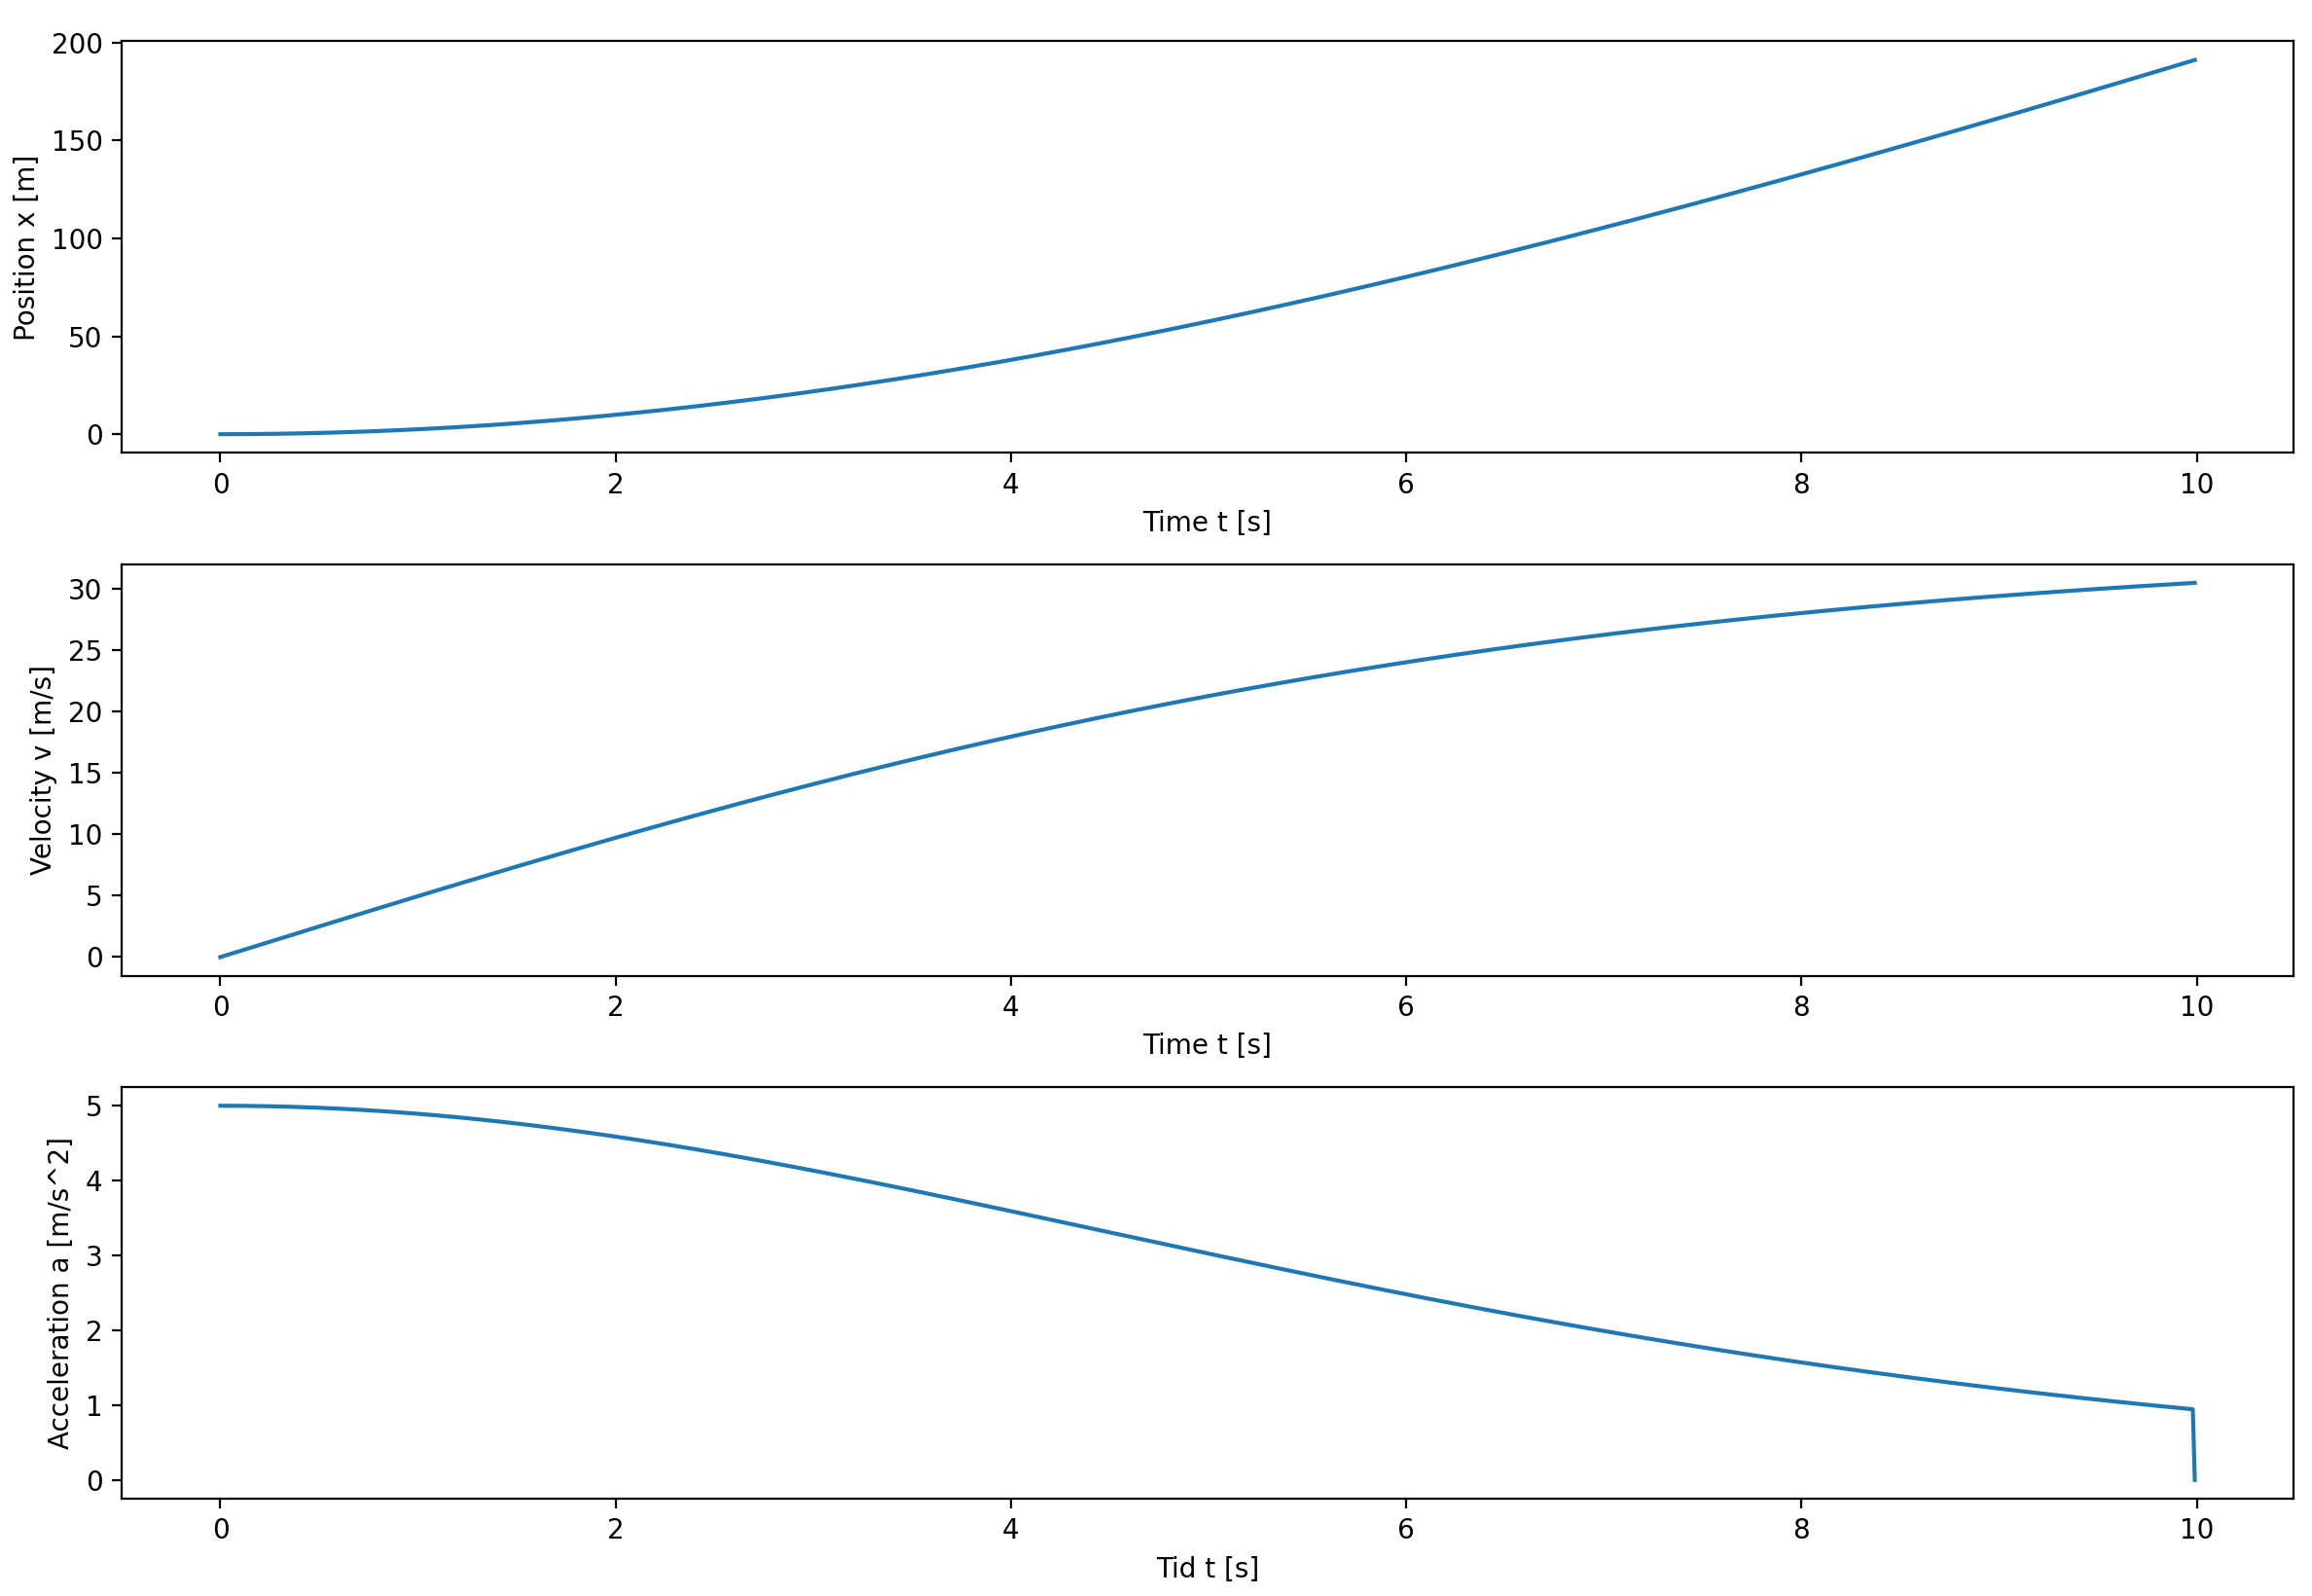
\includegraphics[width=1.2\textwidth,left]{../../graphs/sprinter.png}

            \clearpage

        \subsection*{The second modeling of the runner with other forces added:}
            \lstinputlisting[language=Python]{../../sprinter_2.py}

            \clearpage
        
        \subsection*{The new graph for the runner}
            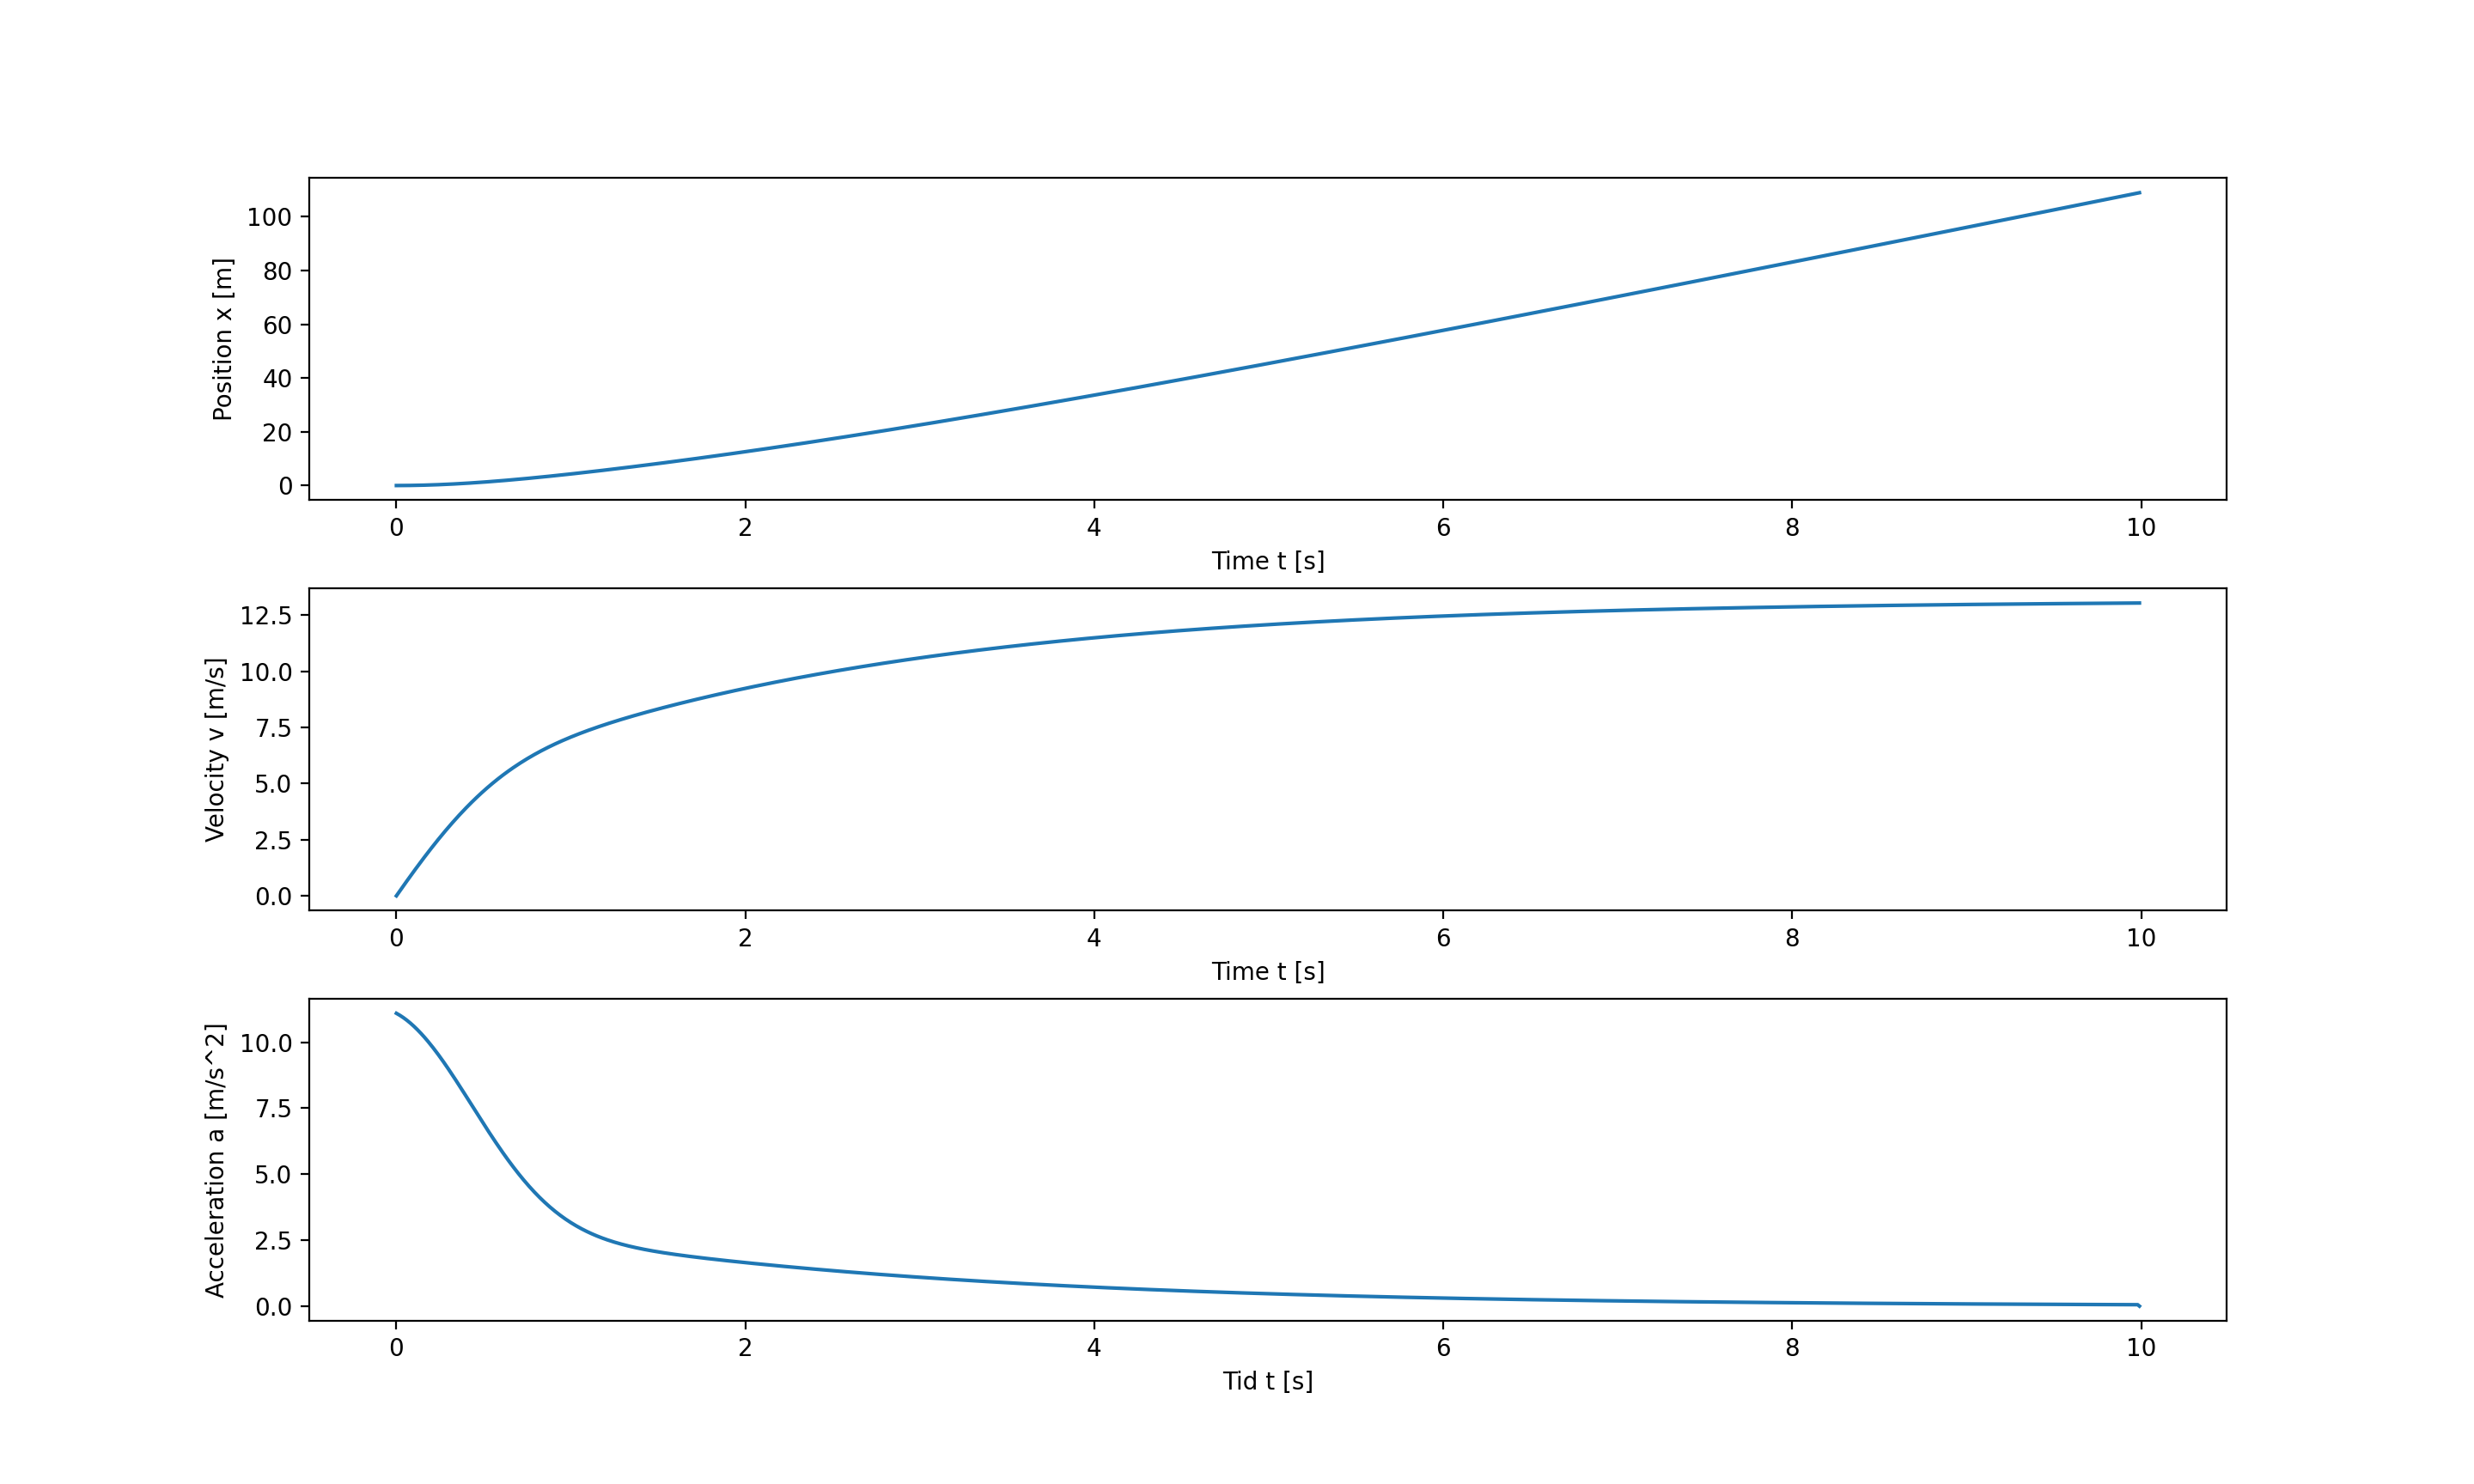
\includegraphics[width=1.2\textwidth,left]{../../graphs/sprinter_2.png}
            
\end{document}